\chapter{Introduction}\label{chap:introduction}


This section will discuss the research questions and the research approach of the
thesis, as well as the motivation behind it.

\section{Motivation}

Artificial intelligence (AI) has entered various industries during the past few years, including the automotive sector. From advanced driver assistance systems to Tesla's autopilot, AI is used to improve traffic safety. Testing autonomous vehicles in actual traffic situations would be risky, defeating the goal of assuring safety.

As a result, simulations are used to test autonomous vehicles. These simulations are created by generating roads and environments to analyse the cars' behavior. Most existing approaches for road generation rely on domain models and metaheuristics. They are limited to generating 2D roads with fixed layouts. These problems could be solved using generative AI.

Generative AI is a branch of Artificial Intelligence that focuses on creating new content. With the use of large language models like ChatGPT \cite{ChatGPT}, there is potential to generate virtual roads for testing by providing verbal descriptions such as "mountain road" or "highway". The output of ChatGPT can then be automatically translated and passed into driving simulators.

\section{Research Questions}
The primary objective of this thesis is to answer the following research question.

Research Question 1 (RQ1): Can generative AI be used to automatically create three-dimensional roads for testing autonomous vehicles?

By harnessing the capabilities of generative AI, the tool streamlines the process of generating roads for self-driving vehicles, eliminating the necessity for complex algorithmic coding.


\section{Research Method}
The research approach consists of four main phases: a review of the state-of-the-art project, implementation of the project, and data gathering and analysis of the data. The findings of the state-of-the-art will serve as a basis for the implementation of the project.

The implementation can be divided into four parts that build on each other. The first part consists of prompt engineering (see section \ref{prompt engineering}) and receiving the output in a format that can be used in the next part. In the second part, a Python script will translate the output into road nodes and interpolate the road. The third part consists of validating the correctness of the road (steepness, sharpness of turns, etc.). The fourth part is building the road in the simulator. The roads will then be evaluated in the context of a user study. 

The quantitative data gathered through the validation script and the user study will then be used for a statistical analysis of the results.

\begin{figure}[ht!]
	\centering
	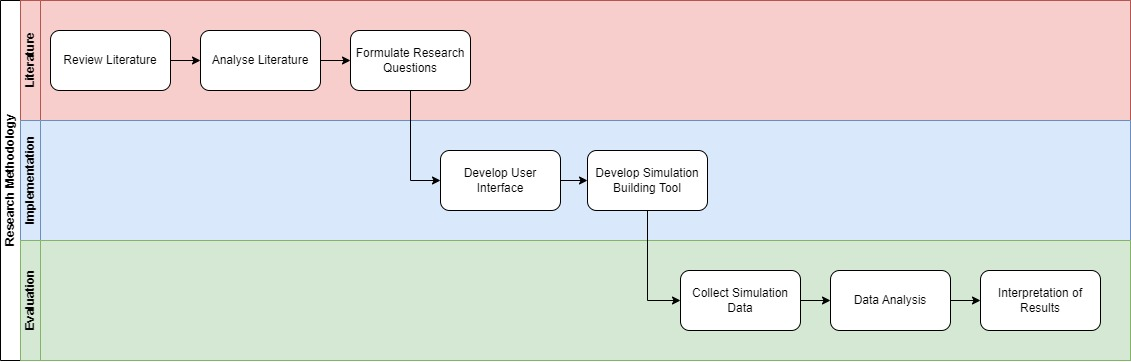
\includegraphics[width=1\linewidth]{images/Research_Methodology.jpg}
	\caption{Research Methodology \label{research methodology}}
\end{figure}

\section{Structure}
The bachelor thesis is structured as follows:
\begin{itemize}
	\item Chapter 1: Introduction

 
    The opening chapter of this bachelor thesis holds significant importance in setting the stage for the research. Within this section, I provide a thorough outline of the motivation driving the study, articulate the fundamental research questions, and present a concise overview of the chosen research methodology. By elaborating on the motivation, the significance and relevance of the study in a broader context is established. The formulation of research questions provides a clear roadmap, guiding readers through the central inquiries shaping the investigation. Furthermore, a comprehensive discussion of the selected research methodology offers insights into the tools and approaches used to address the research questions. This chapter serves as an essential guide, laying the foundation for subsequent chapters and contributing to the overall coherence and clarity of the thesis.
	
	\item Chapter 2: Background
	
	This chapter provides a thorough background that explains the domains and technologies related to the topic. Its primary objective is to supply readers with an overview and the essential vocabulary necessary for understanding the following chapters. By exploring relevant domains, this section seeks to place the research within a broader context, providing the foundation of the study. Additionally, an examination of related technologies is conducted to acquaint the reader with the tools and methodologies essential to this research.
	
	\item Chapter 3: Related Work
	
	The "Related Work" chapter forms a critical component of this bachelor thesis, offering a comprehensive analysis of existing literature and research relevant to the subject matter. In this section, a thorough review of the current state of the art within the field is conducted, examining scholarly contributions, methodologies, and findings that are directly connected to the research objectives. By critically evaluating the existing body of work, gaps, trends, and debates in the literature can be identified. This structured examination of the related work is crucial for establishing the academic foundation of the thesis and demonstrating the unique contributions of the research.
	
	\item Chapter 4: Methodology
	
	This chapter provides a comprehensive overview of the methodology used in this thesis. It offers detailed insights into the systematic approach taken to address the research questions. The chapter covers the research design, data collection methods, and analytical techniques employed, aiming to bring clarity to the procedural aspects of the study. By outlining the methodology, this section not only serves as a guide for potential replication but also establishes the credibility and robustness of the research, laying a solid foundation for the subsequent analysis and interpretation of findings.

    \item Chapter 5: Implementation
    
    Chapter 5 focuses on the practical implementation of the project, explaining how the code works and which technologies were used. It provides a detailed explanation of the project's technical aspects, including the software tools and programming language utilized. This chapter aims to offer readers a clear understanding of how the project was implemented.

    \item Chapter 6: Evaluation
    
    The "Evaluation" chapter serves as a comprehensive exploration of the methods used for assessing the tool's effectiveness. It extensively discusses the procedures used for data collection, analysis, and interpretation. Additionally, it provides a detailed exploration of the user study used to evaluate the tool, covering its setup and execution. Through a thorough examination of these elements, the chapter aims to offer a comprehensive understanding of the evaluation process and provide insights into the tool's performance.
	
	\item Chapter 7: Summary
	
	This chapter presents the main findings of the study. The insights obtained from the results are presented by systematically analyzing and interpreting the collected data. The findings are discussed in detail, highlighting their relevance to the research questions and objectives.
\end{itemize}